\documentclass{standalone}
\usepackage{pgfplots, gensymb}
\pgfplotsset{compat=1.7}

\begin{document}
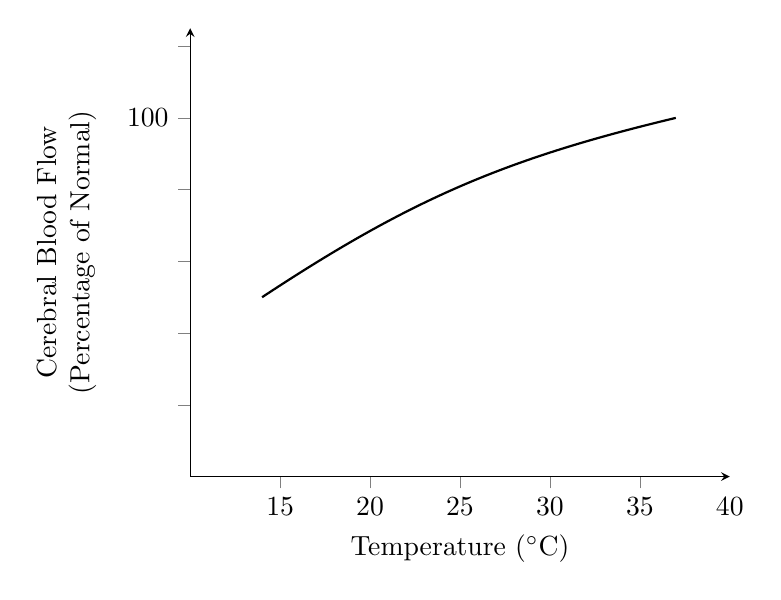
\begin{tikzpicture}


\begin{axis}[
        axis lines=middle,
        grid = none,
	ymin = 0,
	ymax = 125,
	xmin = 10,
	xmax =40,
	 ylabel near ticks,
	xlabel near ticks,
	extra y ticks={100},
	yticklabels={},
	        xlabel=Temperature ($^{\circ}$C),
        ylabel=Cerebral Blood Flow \\ (Percentage of Normal),
        tick align=outside,
        enlargelimits=false,
ylabel style={align=center},
legend pos= north west,
legend style={font=\small, cells={align=left}}]

\draw[thick, black] (axis cs: 37, 100) to [bend right=10] (axis cs: 14, 50);

\end{axis}

\end{tikzpicture} 
\end{document}